\chapter{Discussion}\label{sec:discussion}

In this chapter, we discuss advantages and disadvantages of the different 
models developed  and compared to in this thesis, and justify our 
contributions. In addition, we address possible criticisms and other tradeoffs 
and design choices that are of importance beyond pure accuracy.  Performance of 
the different models in terms of part localization accuracy is 
in~\secref{system-results}.

\section{The case for image-dependent interactions}

At the time of publication, CPS was significantly better than all modern ``in 
the wild'' pose estimation approaches 
\citep{ferrari08,eichner09,devacrf,andriluka09}.  CPS was the only one to use 
image-dependent pairwise cues.  These other systems focused on either 
pre-processing to reduce the state space or improving unary potentials via 
foreground color estimation, and all performed inference relying ultimately on 
edge-based unary potentials and simple geometric displacement pairwise cues as 
in the classical PS model (\secref{ps}).
\out{
Recently, \citet{deva2011} introduced a multi-modal model of pose that competes 
with CPS. However, empirical results indicate that CPS generalizes better than 
\citet{deva2011}: when both models are trained on Buffy, CPS outperforms 
\citet{deva2011} on Pascal. Furthermore, two years after its introduction in 
the literature, CPS is still the best performing model in the less precise 
regime (\figref{results-buffy-pascal}).  One of the reasons for the lack of 
precision is the coarser nature of our features: whereas \citet{deva2011} can 
evaluate placements to the granularity of a HoG cell, many of our features are 
more coarsely described and/or discretized---\eg, is the part guess near a 
contour, is the part guess in the foreground color.
}
In a controlled setting, we see that a classical PS model coupled with just one 
image-dependent interaction feature, such as contour continuity, significantly 
improves performance (\figref{ablative}).  This makes a strong case that 
image-dependent interactions improve performance.

The benefits of image-dependent interactions is further reinforced by the 
performance by our video pose estimation model.  The Ensemble of Stretchable 
Models exploits a variety of across-body and across-frame image interactions 
and significantly outperfoms methods with fewer interactions.

Finally, we see effective data-dependent switching of modes in our LLPS model.  
The decision of which local model $s^z(x,y)$ to choose depends on large-context 
interactions considering a whole half-body in scope. These holistic cues are 
crucial in determining an effective mode to use, and serve as one of the main 
reasons LLPS outperforms~\citet{deva2011}.

We believe our cascade approach is a very useful tool that helps us design 
models with larger image-dependent interactions.  It is a key component to all 
models presented here to achieve a high degree of accuracy and/or efficiency.  
The cascade framework also holds potential to improve the richness of models in 
the future.  In general, our approach is a principled framework that frees us 
from restricting our models to limited pairwise potentials of the form $||y_i - 
y_j||$.  This allows much more flexibility in the future to incorporate more 
pairwise and even higher-order features. 

\section{More features or more modes?}
As discussed in~\secref{llps}, there are two major approaches for improving 
pose accuracy in recent years: adding more features, \eg CPS, ESM and 
\citet{ferrari08,eichner09,ddtran}, or adding more modes, \eg LLPS and 
\citet{dpm,wang2011,deva2011,everingham2011}.  

LLPS and~\citet{deva2011} are both multimodal models that outperform the 
feature- and computation-heavy CPS.  It is unclear given the current 
state-of-the-art if the multimodal HoG model approach is yet saturated, or more 
data and more nuanced mode definitions will continue to yield increased 
performance in coming years.  \citet{zhuwe} has an excellent study of whether 
these models are near saturation; see \figref{llps-learning-curve} for our own 
trend analysis.  Both suggest that we are not near saturation yet, in terms of 
number of parts, modes and training data. There are also no limit to the 
performance gains to be had by adding more and better features, only 
computational hurdles.

\begin{figure}[htb!]
\centering
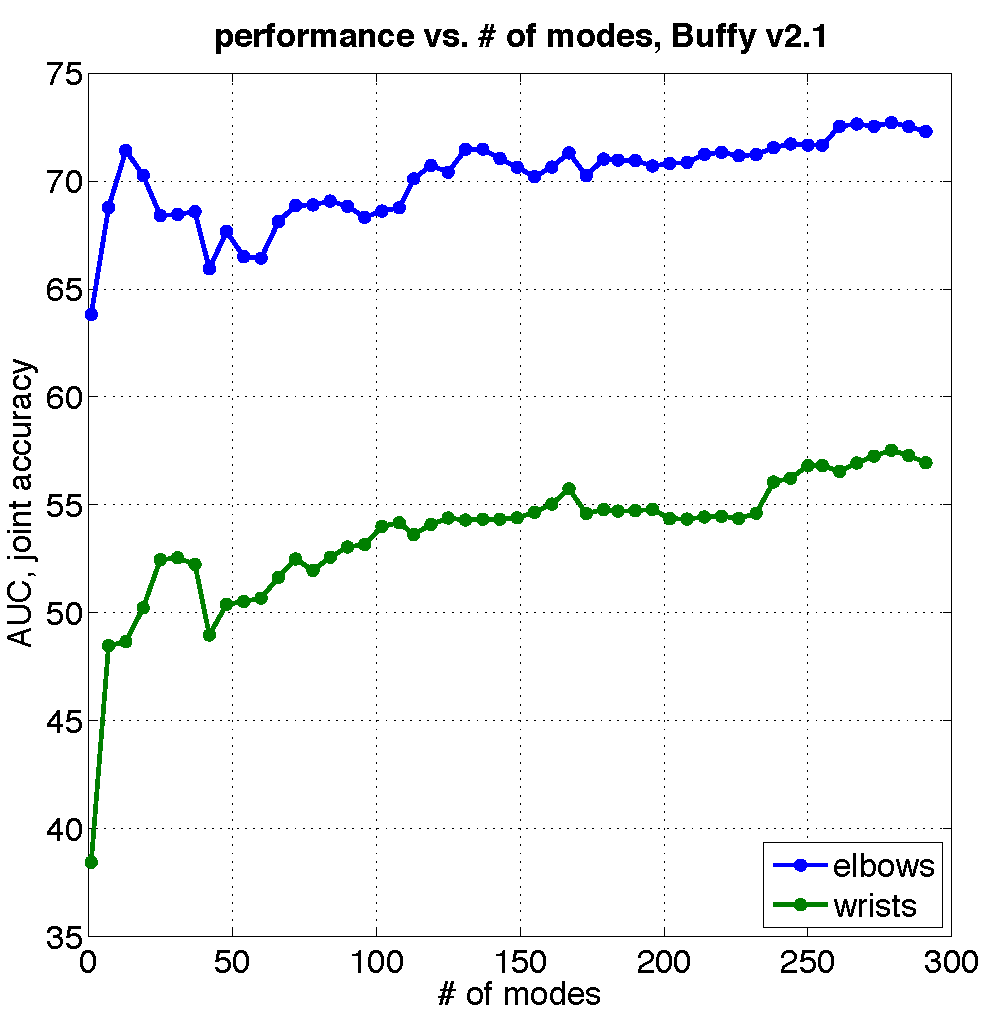
\includegraphics[width=0.70\linewidth]{figs/llps-learning-curve.pdf}
\caption[LLPS learning curve.]{
\label{fig:llps-learning-curve} LLPS learning curve: test set accuracy for 
wrists and elbows combined for LLPS models trained with different amounts of 
data.  The mode definitions, number of modes, and cascaded mode prediction step 
were held fixed and used for training.  }
\end{figure}


Ultimately, these research directions are complementary, and an ideal model 
would use a combination of rich features and multiple modes. Each additional 
feature type (\eg, segments, contours, optical flow, depth) incurs an 
additional cost to obtain, but adds to the generalization capabilities of the 
model. Additional modes allow for more specific modeling of different 
scenarios, but require more training data to estimate parameters accurately.  
This leaves a large space of possible models combining the two approaches.

\section{Joints or limbs?}

The ESM model introduced a joint-based 2D representation of pose.  At the same 
time, \citet{deva2011} also introduced a model based on joints and limb 
midpoints as basic units of inference.  This approach has clear benefits for 
easily capturing foreshortening and scale.  It has the seeming disadvantage of 
not being able to capture limb-pair features with a pairwise model.  However, 
this is not a fundamental limitation.  Especially using cascaded inference 
techniques we should not shy away from describing higher order cliques in the 
future.  In general, the scope of the basic atomic unit for inference (the 
inference variables) need not be dictated by the scope of the largest clique we 
capture in our model.  Joint-based models are worth exploring further.  In 
particular, we expect an Ensemble of Stretchable Models approach applied to 
{\em single frame} pose estimation to work well.

\section{Detection, localization, or both?}

Some pose estimation systems advertise that they work well for both person 
detection {\em and} pose estimation---in particular \citet{andriluka09} and 
\citet{deva2011}.  One system that does both is beneficial in its 
simplicity---one function to both find a person and find their body parts.  Our 
approach, on the other hand, requires first detecting a person with a dedicated 
person detector, and then running our pose models on the detected person. 

We believe that detection and localization are fundamentally different tasks 
and should be decoupled.  In detection, we wish to generalize over all poses 
and determine how to discriminate any pose from background clutter---a 
detection is correct even when a pose is incorrect, and a detector must also 
have some notion of global confidence to determine, over all possible image 
patches, whether it is a person or not.  A pose estimator works under the 
assumption that a pose is present, and is correct only if it predicts the right 
pose versus combinatorially many wrong poses.

One model that attempts to perform both tasks is bound to perform only as well 
as it could tuned to each task independently, and probably worse.  It may be 
that PS models are the right {\em family} of models for both detection and 
localization---they have attractive benefits for generalizing over poses with 
deformations and obstructions in addition to localizing pose---and they should 
be used for both.  However, models should be trained evaluated specific to a 
single task.

\section{Everything and the kitchen sink: a bug or a feature?}
One of the selling points of our models is the ability to include a multitude 
of features.  The goal is to include as many feature modalities as possible in 
our CPS and ESM models.  Having so many features makes it difficult to 
determine exactly what is contributing to the success of our model.  

From a machine learning standpoint, this is an attractive aspect of our system: 
given training data, we can try everything and see what works.  From a computer 
visionist's (or perceptual scientist's) perspective, this is a 
disadvantage---it is difficult to gain insight into why the model is performing 
well.

We take a functional, application-driven approach towards computer vision, and 
consider our problem one of engineering rather than perceptual science.  The 
inability to measure the individual performance of components in any complex 
system is inevitable---the whole is greater than the sum of its parts.  We 
provide individual feature analysis in~\figref{ablative}, and make convincing 
arguments that the features and interactions we include are beneficial.  We 
make no statement as to which features are the ``best'', in any sense other 
than their contribution to final system performance.

\section{Accuracy, speed, simplicity}
\begin{figure}[htb!]
\centering
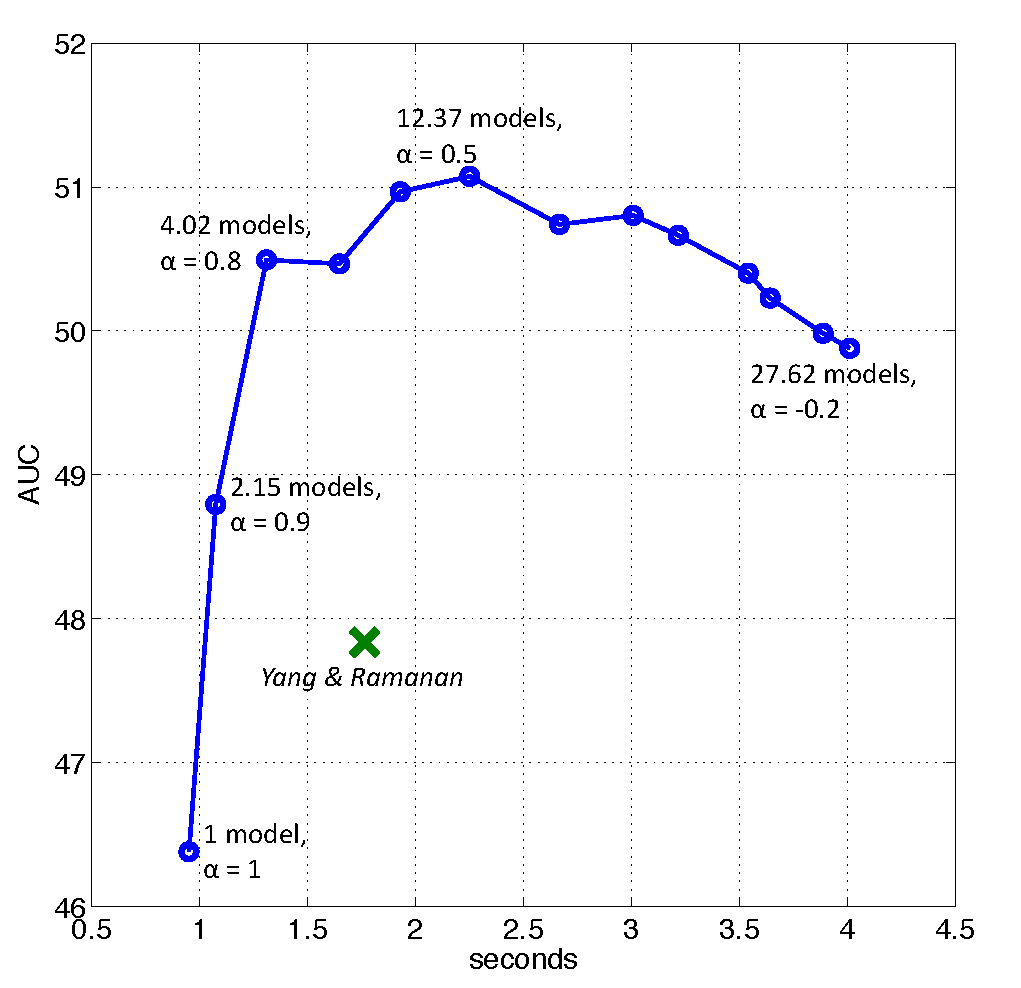
\includegraphics[width=0.95\linewidth]{figs/speed-vs-acc.pdf}
\caption[Speed versus accuracy.]{
\label{fig:speed-v-acc} Test time speed versus accuracy.  Accuracy is measured 
as area under the pixel error threshold curve (AUC).  Speed is in seconds on an 
AMD Opteron 4284 CPU @ 3.00 GHz with 16 cores.  On the left, we compare 
different methods with a log time scale.  The upper left corner is the most 
desirable operating point.  LLPS is strictly better than other methods in the 
speed-accuracy space.  On the right, we zoom in to investigate our cascaded 
LLPS approach.  By tuning the aggressiveness ($\alpha$) of the cascade, we can 
get a curve of test time speed-accuracy points.  Also, we see that ``full 
training''---considering all modes in every training example---rather than
``cascaded training''---just the ones selected by the cascade step---leads to 
roughly a $1.5\%$ performance increase (at the cost of $5\times$ slower 
training).}
\end{figure}

When developing our CPS and ESM models, we focused our attention on obtaining 
the best performing, computationally tractable system.  Besides raw 
performance, practitioners care as much about {\em speed}---does the system run 
quickly?---and {\em simplicity}---how long does it take to download, compile, 
understand, run and/or re-implement?  One of the motivations of LLPS and 
attractiveness of~\citet{deva2011}'s model is its speed and simplicity, in 
terms of image features (only HoG) and lines of code.

LLPS is strictly better than other models in terms of speed and simplicity, 
according to \figref{speed-v-acc}. \citet{deva2011} is strictly better than all 
but LLPS.  Among the other models, there is no clear winner---CPS is more 
accurate but slower.  Predicting cluster means is extremely fast but less 
accurate.

We believe that, moving forward, models with any combination of the three 
contributions {\em accuracy, speed, simplicity} are all worthwhile, even 
independent of the others. Any current system's slowness today will likely be a 
non-issue in 5-10 years with the advent of faster CPUs and more cores.  
Anecdotally, at time of publication two years ago, the CPS system took 5 
minutes and 15 seconds.  Today, at roughly the same price and consumer 
availability, the system runs in 3 minutes.


\chapter{Future directions}
{\small
{\em \begin{enumerate}
  \setlength{\itemsep}{1pt}
  \setlength{\parskip}{0pt}
  \setlength{\parsep}{0pt}
\item When a distinguished but elderly scientist states that something is 
possible, he is almost certainly right. When he states that something is 
impossible, he is very probably wrong.
\item The only way of discovering the limits of the possible is to venture a 
little way past them into the impossible.
\item Any sufficiently advanced technology is indistinguishable from magic.
  \setlength{\itemsep}{16pt}
\item[---] \text{Clarke's Three Laws, Arthur C. Clark}
\end{enumerate}
}
}
\line(1,0){250}
\vspace{0.5in}

In this chapter we suggest avenues for further research, both in pose 
estimation and other domains in computer vision and machine learning.  Some of 
it is speculative.  Our hope is that the work of this thesis is a building 
block for these new research directions in the near future. 


\section{Solving pose estimation}

What would it take to declare pose estimation solved?  Certainly with current 
accuracies---getting wrists right about half the time---we cannot claim that 
the state-of-the-art ``works,'' from a layperson's perspective.  Taking a 
functional standpoint, we deem to call pose estimation solved when it is ready 
to be featured in a consumer product in the wild, the way face detection is in 
cameras and the Kinect now in video games.  We speculate that accurately 
localizing elbows and wrists $90\%$ of the time in datasets like MoviePose 
would be sufficient for this level of broad use.  However this would still 
leave enormous room for improvement---MoviePose and our current models do not 
consider handling multiple people and their interactions or reasoning about 
occlusion or very non-frontal non-upright poses.

As a side note, our current state-of-the-art in pose estimation may very well 
be ready to be used as a second-tier method in real-world applications, in the 
sense that the pose output is not relied upon, but is treated as a non-crucial 
but helpful noisy sensor.  \citet{wang2011}, for example, use it as a 
descriptor for action recognition. The same is done for image retrieval 
\citep{posesearch} and scene geometry estimation \citep{gupta11,delaitre12}.


\subsection{Pushing current models to their limits: more data, more modes, more
submodes and supermodes}

\begin{figure}[tb!]
\centering
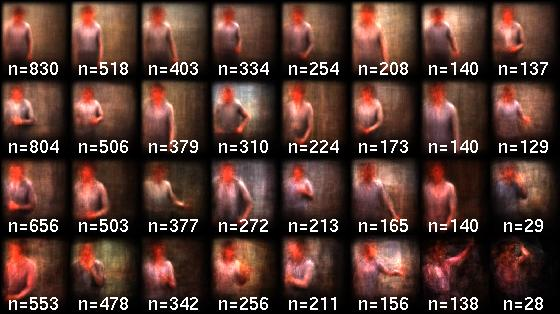
\includegraphics[width=0.99\linewidth]{figs/llps-modes.jpg}
\caption[LLPS modes and counts.]{
\label{fig:llps-modes-counts} LLPS mode image centers and their population 
counts, populated by MoviePose. }
\end{figure}

  How might we achieve higher accuracy on MoviePose?  The superficially 
uninteresting but most promising way forward is using the same models, but with 
significantly more data.  Currently, LLPS is comprised of 32 mode models, which 
cover the range of human pose in video quite well.  The most common mode (arms 
at rest) has 800 training examples at its disposable; the least common modes 
(arms raised above head and hand held up to face) have less than 25 examples 
each.  See \figref{llps-modes-counts}.  Immediately we see there is room to 
flesh out some of the rarer categories and estimate them better.  

As a back-of-the-envelope calculation, to collect enough data to train the 
least frequent mode with 500 examples, respecting the natural mode distribution 
collected from movies, we would need twenty times as much data.  In addition, 
although 32 modes cover the variations in upper body pose well, we expect to 
get more accurate modeling by also considering modes of appearance, from 
clothing and body type.  From intuition, it seems reasonable that each of our 
current 32 modes could be split into at least 3 submodes based on 
appearance---for example, one submode for men's arms, one for women's, and one 
for baggy clothing.  This would bring up the tally of data needed to 60 times 
the current levels, for the least frequent modes to be modeled with 3 submodes, 
each with 500 training examples.

It is almost flippant to suggest simply using more data will solve our 
problems.  First, obtaining and labeling this data is no small feat; difficult 
but not impossible.  Second, careful methods to train on such large datasets 
need to be designed.  \Naively using current training methods for 60 times more 
data would result in 13 days to train and would require 1.4TB of memory; 
slightly out of the realm of feasibility for current standard servers.  

A final problem is that scaling up to a larger number of classes always tends 
towards more class confusion.  This is a much more studied issue in large 
classification tasks such as the ImageNet retrieval challenge \citep{imagenet}, 
in which 10,000 different classes are to be predicted.
A common way to deal with class confusion at large scale is hierarchical 
classification, \eg first predict non-animal from animal, then dog from other 
animals, then Corgi from Bernese Mountain Dog.  The hierarchical decisions are 
easier to make and there are less of them than comparing all fine-level 
classes.  This suggests an analogous approach to multimodal pose modeling: 
group the 32 modes recursively into 16, 8, 4 and 2 coarse supermodes.  Cascaded 
prediction could also be effectively applied here.

In summary, to push the current LLPS model framework to its limits, we require 
at least an order of magnitude or more additional data, cleverer training 
algorithms (or patience), and a richer hierarchy of modes, some more specific, 
some more general than our current collection, based on both pose and 
appearance.  It is our belief that such improvements to our model could enjoy 
incredible leaps in performance in the coming years.  Preliminary studies on 
pushing the state-of-the-art of multimodal models with increasing data and 
modes in other domains has similar conclusions \citep{zhuwe}.

\subsection{Putting people in their places}

\begin{figure}[tb!]
\centering
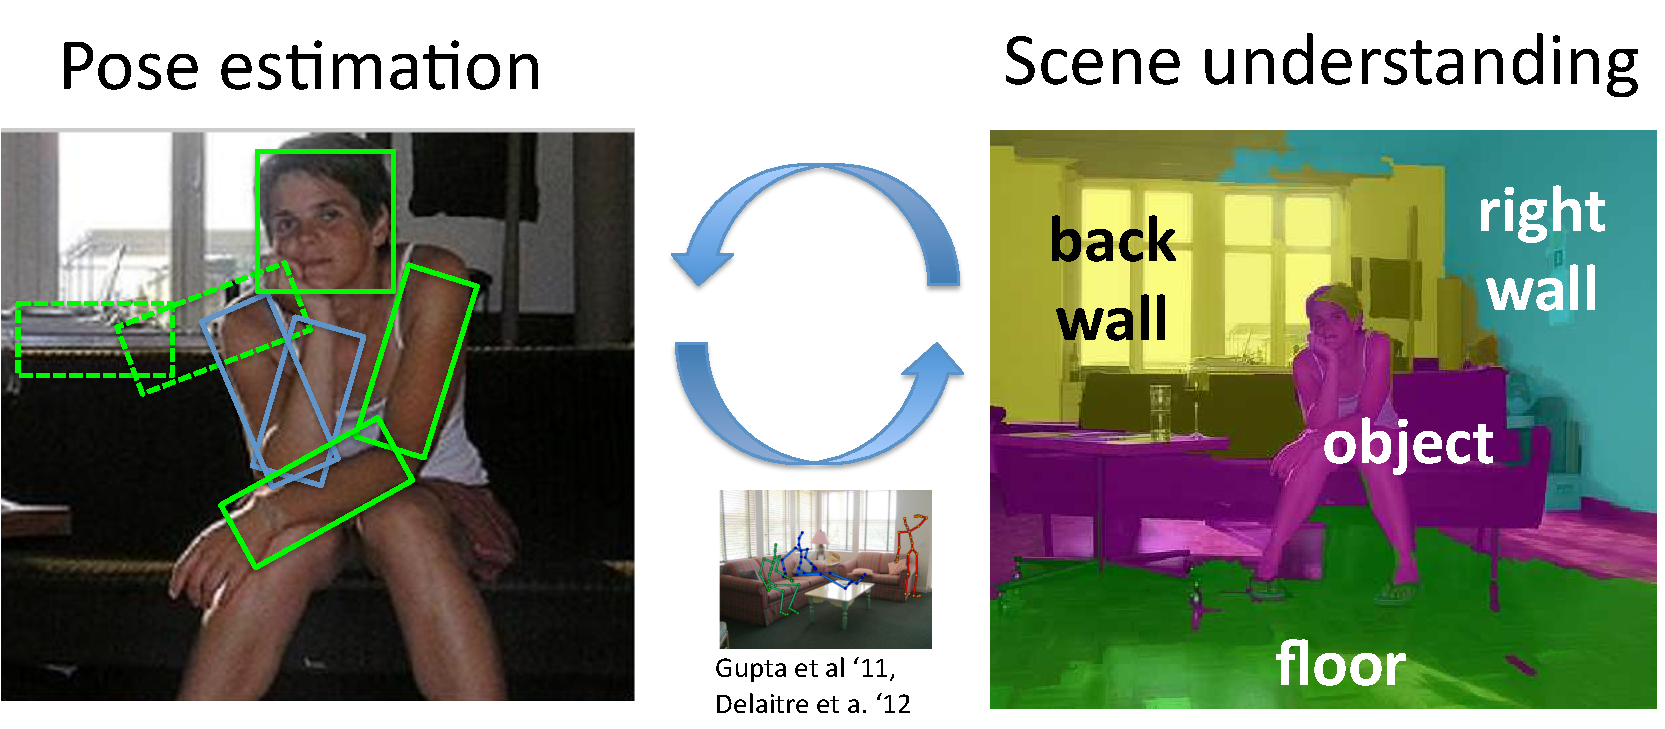
\includegraphics[width=0.80\linewidth]{figs/pose+scene.pdf}
\caption[Joint pose and scene reasoning.]{
\label{fig:pose-scene} {An illustration of how scene parsing and pose 
estimation can aid each other. \citet{gupta11,delaitre12} have shown that 
state-of-the art pose estimation helps infer scene geometry.  We believe that 
scene parse information (such as that by \citet{lee09} run on the image on the 
right), can help pose estimation, \eg, by indicating that the true arm location 
(blue rectangles) are more likely than the false positive in the background 
(dotted green rectangles). }}
\end{figure}


We believe pushing multimodal models to their limits in the coming years will 
bring a high degree of accuracy to frontal upper body pose estimation.  Even 
so, these models leave much to be desired.  Importantly, they are unable to 
reason about occlusions and multiple people. 

Some methods in the past model occlusion probabilistically, however, the basic 
reasoning essentially boils down to a threshold on the lack appearance evidence 
for a part~\citep{wang2008multiple}.  As we have shown throughout this thesis, 
the decision to make about an arm not being present versus just being difficult 
to detect (in which case we should just make a best guess) is extremely 
difficult with current models.  In reasoning about multiple people, 
\citet{eichner2010we} explore the combinatorially many possibilities of 
detected people in a scene, \citet{kulesza11} provide a framework for sampling 
a high-quality, diverse set of poses, and \citet{andriluka-multiple} model 
interacting people by connecting them together in one tree-structured PS model.

In all the above models, we believe a key missing ingredient is the context 
around the person.  Pose models to date only try to separate pose from 
background, and there is attempt to understand or explain the background.  We 
envision a model that attempts to put people in the scene around them, and 
label every pixel in the scene along with it, similar to standard scene 
parsing.  

We believe modeling the scene and pose jointly is crucial to determining 
whether a part is occluded: it can consider as evidence whether there is an 
occluding foreground object, not simply declare occlusion whenever the part 
detector signal is weak. Similarly, multiple people can be explained and 
reasoned about as explicit objects. 

\citet{gupta11,delaitre12} have already provided empirical evidence that 
current pose estimators can aid scene geometry and scene labeling inference.  
We believe the other direction is also true: scene models can help pose 
estimators.  A simple proof-of-concept is demonstrated in \figref{pose-scene}.  
There is much interesting work to be done reconciling pose and scene models to 
agree, and what their lingua franca representation should be.  Agreement 
algorithms such as those discussed in \secref{stretchable} may be quite viable 
here.  As a starting point, \cite{koller11} propose a simple model that coupled 
a figure-ground segmentation model with a PS model, with modest performance 
improvements.
 
\section{Pose models on other problems}

Pose estimation is a challenging problem with fundamental computational 
complexity issues.  The methods developed in this thesis may well be applied to 
other important and challenging problems in computer science.  We discussing a 
few promising ones here.

\subsection{Bringing cascades to the masses}
The application of structured prediction cascades has already been successful 
in a variety of domains besides pose estimation: optical character recognition, 
part-of-speech tagging \citep{cascades-jmlr} and natural language dependency 
parsing \citep{slav-naacl}.

There are several structured problems in computer vision which contain similar 
computational bottlenecks, and as result settle for models with restricted 
forms of part interactions.  One is \textbf{scene parsing}, in which each 
segment of an image must be labeled with one of a handful of labels.  Because 
of the cyclic graph structure, only simple neighbor interactions are studied.  
Recently, \citet{munoz10} showed that a non-structured hierarchy of models 
which captured large part interactions proved to be very effective.  We expect 
that applying a cascade to this problem would allow us to keep both the nice 
properties of a structured model as well as the benefits of data-dependency in 
large cliques of segments in an image.

Similar trends can be seen in the \textbf{optical flow} literature, which poses 
the correspondence problem between a pair of images as a structured prediction 
problem with a data-independent pairwise smoothness term.  Good results are 
currently achieved \citet{liu2011sift}, who use a coarse-to-fine approach to 
speed up the matching.  Cascades would provide a principled way to do this, as 
well as incorporate data-dependent smoothing terms---for example it could 
depend on local texture or permit sharp changes at strong boundaries.

\textbf{Image retrieval} systems typically follow a paradigm of (1) obtain a 
short list of possible candidates for retrieval using cheap and coarse nearest 
neighbor search via bag-of-words descriptors, and (2) perform more 
computationally intensive matching on the short list 
\citep{wang2011contextual}.  This is a heuristic two step cascade.  We envision 
a progression of cascade models that operates on histograms of bags of words, 
then histograms of word bigrams, then trigrams, etc. With larger n-grams we 
hope to use richer word frequency and spatial consistency cues to get better 
results.  The finer cascade progression and learned accuracy-efficiency 
trade-off we hope would also yield better performance.

Scaling up to many various applications, one is compelled to think of 
\textbf{automatically building cascade architectures}.  Designing structured 
prediction cascade applications thus far has been accomplished manually based 
on domain expertise---determining how the state space should be refined, and at 
what stage of the cascade should refinements and additional modeling power and 
complexity be introduced.  In fact, the CPS model cascade architecture was 
designed by intuition and cross-validation in a greedy stage-wise manner.  It's 
unlikely that it has the optimal speed-vs-accuracy tradeoffs compared to the 
introduction of features earlier or later in a cascade, deeper cascades,  or 
different features. The same question exists for the original \citet{viola02} 
classifier.

One promising approach towards automatic cascade architecture design would be 
to provide an algorithm with a pool of cascade refinement elements (from 
features, or state space transformations), each with measurable efficiency, 
accuracy and computation behavior.  It would be the job of the algorithm to 
choose a sequence of elements to build an effective cascade from scratch.  For 
example, in an LPPS-type model, we could give the algorithm a pool of modes 
that span the continuum of coarseness to fineness.  The algorithm could decide 
how many modes to use, what their granularity is, and how to arrange them so 
that at test time inference is efficient and accurate.

This has been studied for binary cascades, for example by 
\citet{lefakis2010joint}, which jointly learns all levels of the cascade to 
achieve better performance than the hand-crafted \citet{viola02} detector.  
These same issues are also of critical importance in applications such as 
medical diagnosis, where the introduction of new features comes at a 
considerable cost (from additional diagnostic tests or adding more participants 
in a clinical study).  In statistics this is known as sequential hypothesis 
testing,  which has been applied to efficiently determining image similarity by 
\citet{ofir-pami}.  \citet{deng11} greedily infer a ``label tree'' for 
efficient classification of a large number of classes.  Lastly, \citet{vanroy} 
learns a decision process model via reinforcement learning.

\subsection{Solving graph problems with tree agreement}
In \secref{stretchable} we propose a simple approximation to minimizing a 
general pairwise energy function with cyclic dependencies---tree decomposition 
with single variable agreement; combining beliefs through max-marginals. In 
this problem, we showed that it was a cheap and effective alternative to dual 
decomposition \citep{komodakis2007}. 

The raises the question of whether the technique can be applied as well to 
other hard graph minimization problems.  These include problems such as scene 
parsing, stereo matching, graph matching, image denoising, optical flow, and 
protein design.  For problems that are relatively easily solved, 
state-of-the-art minimization techniques might be overkill, and single variable 
agreement may be just fine.  For a toy demonstration of this, see 
\figref{constellation-demo}.  Methods such as 
\citet{jojic10,sontag-thesis,batra2011making} are iterative processes with 
approximation guarantees but are considerably slower. 

On problems that are difficult, it may also be the case that our single 
variable agreement may work just well as more sophisticated costly 
techniques---in other words, they all may be far from the global optimum.  It 
remains an open but important question to characterize when single-variable 
agreement may work well empirically and in theory, and what approximation 
guarantees it might admit.


\begin{figure}[p!]
\centering
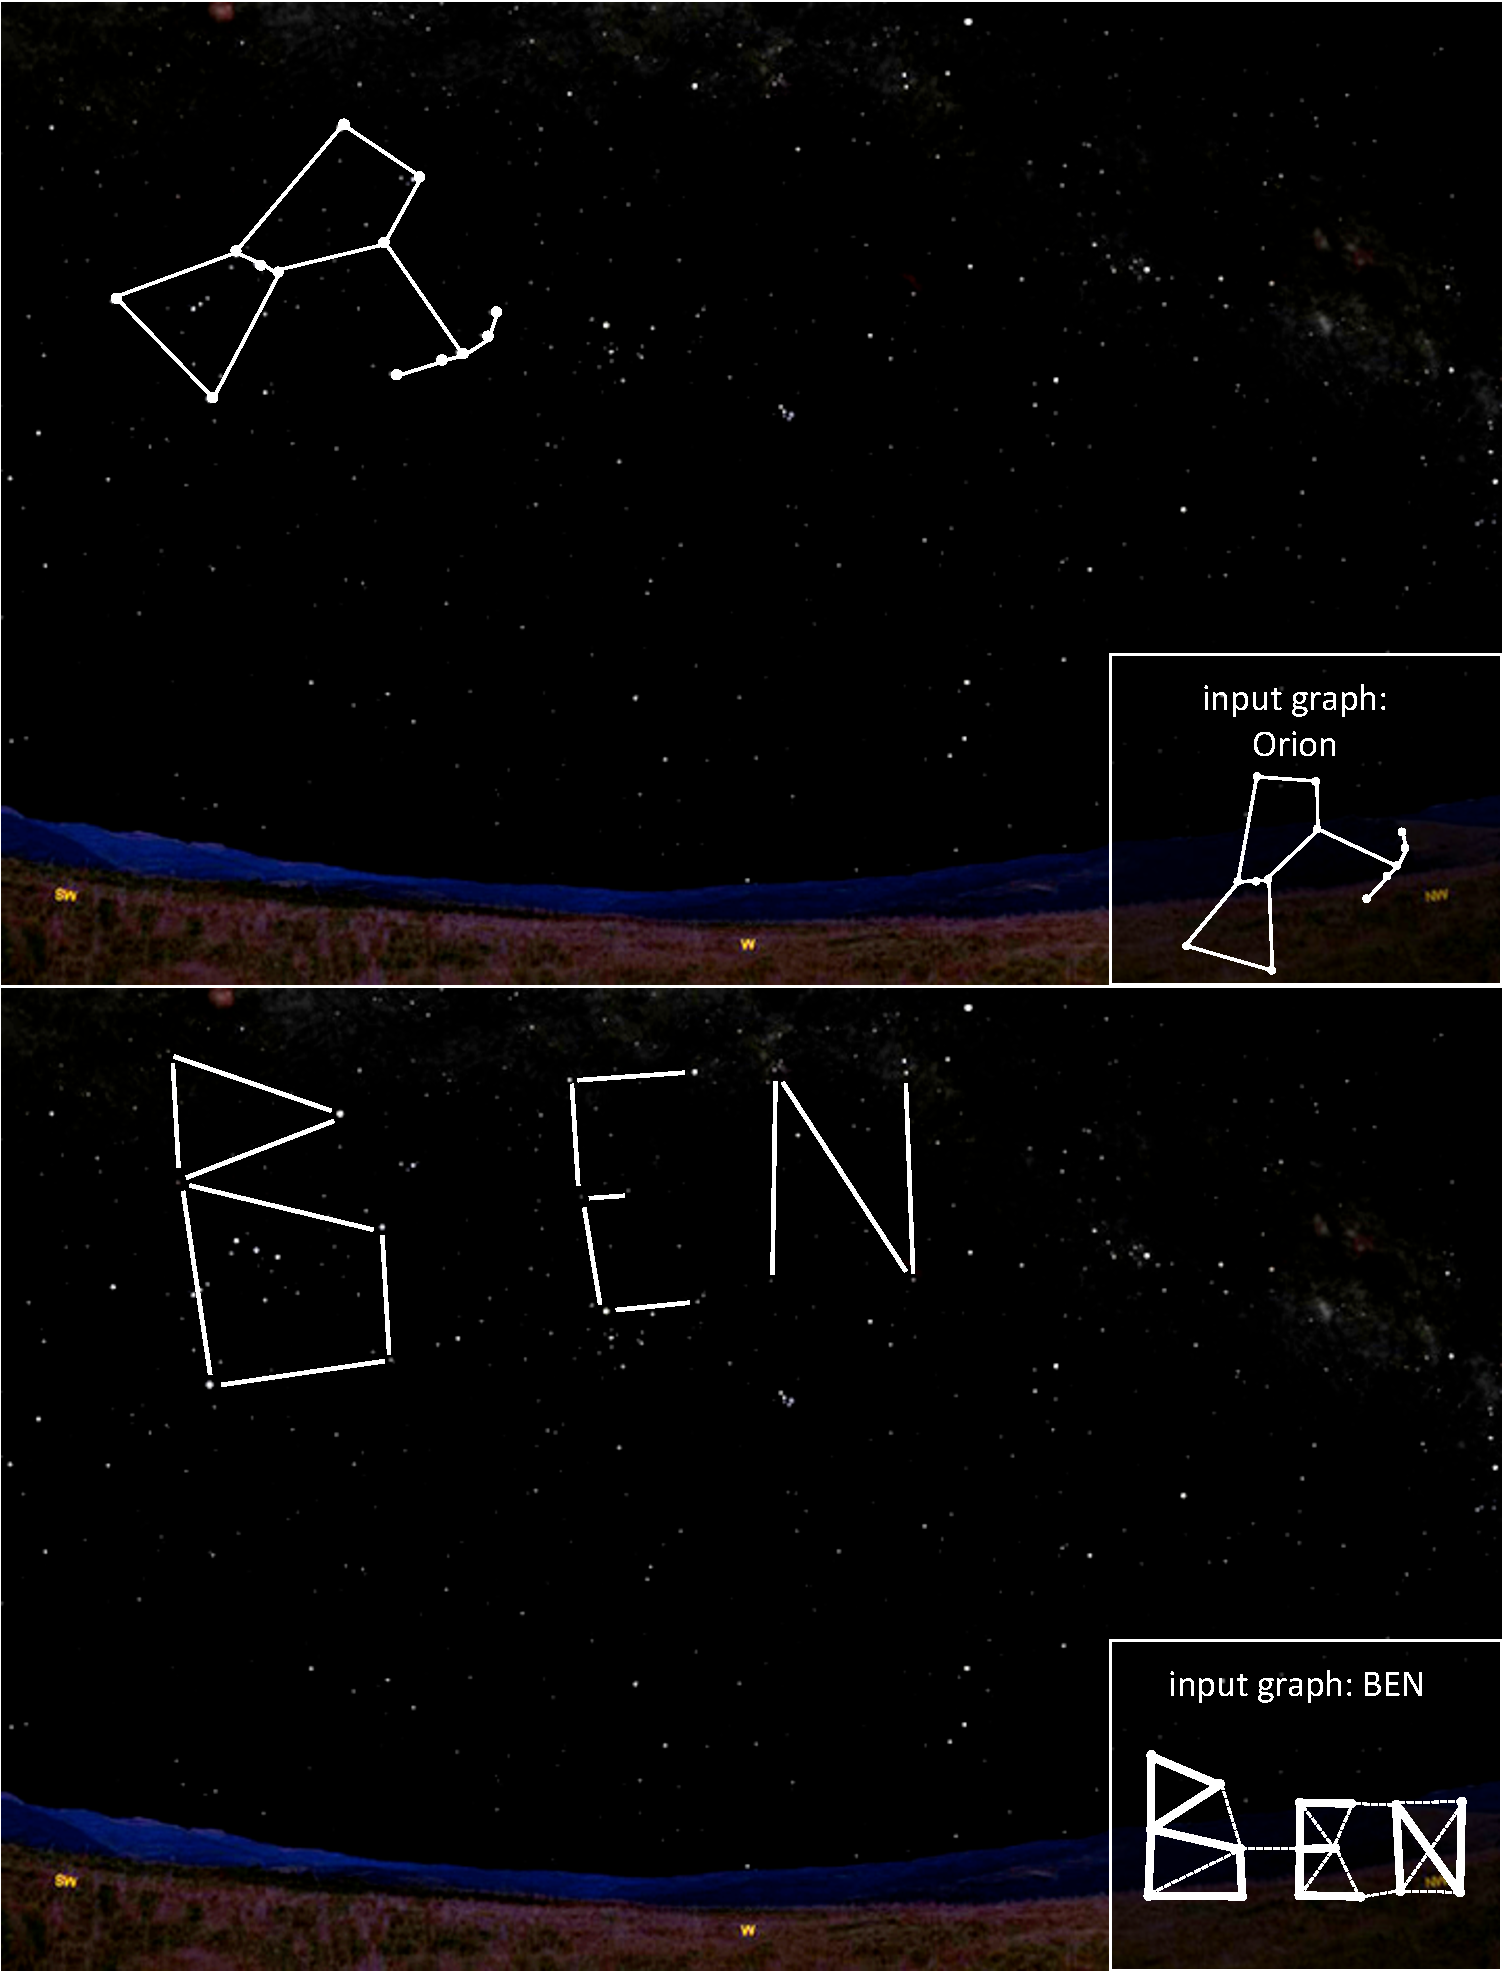
\includegraphics[width=0.80\linewidth]{figs/constellation-demo.pdf}
\caption[Constellation finder app.]{
\label{fig:constellation-demo} {\footnotesize A demonstration of a toy 
application of tree agreement: a constellation finder.  Given a loopy graph 
that defines a constellation's geometric structure, our tree decomposition plus 
variable agreement method (\secref{stretchable}) can match the graph in the 
night sky (state space is the set of star points).  Here we decompose the 
cyclic graph into a collection of spanning trees, one rooted at each node and 
obtained automatically via depth-first search. This method  works both for 
searching known exact geometries like the Orion constellation, as well as for 
discovering new, user-designed constellations.  Note that any single spanning 
tree of these constellation models fails to represent all the important 
geometric connections, and results in false positive matches in practice. }}
\end{figure}


\chapter{Conclusion}

This thesis proposes advancements in 2D human pose estimation models to improve 
upon state-of-the-art performance.  Specifically, previously proposed pictorial 
structures models are handicapped by the needs of efficient inference tricks; 
forced to express simple pairwise cues that are only a function of parts' 
spatial relationships.  Further, the spatial relationship structure had to form 
a tree graph.

We push past the inference barrier in several ways, allowing us to include 
richer image-dependent interactions.  First, we proposed Cascaded Pictorial 
Structures ({\bf CPS}), a sequence of structured models that efficiently prune 
the state space of possible poses down to a manageable number.  This allows us 
to perform efficient exact inference without restrictions.  We exploit this by 
incorporating a variety of rich features from complementary sources, improving 
upon state-of-the-art PS approaches in single frame pose estimation.

We then extend this approach to handle pose estimation in video.  Maintaining a 
rich set of variable interactions in video creates a cyclic network, which is 
known to require inference inference exponential in the number of frames of 
video.  We maintain tractability through the use of a cascade step as in CPS, 
and an approximate inference method which decomposes the cyclic structure of 
interactions into an ensemble of tree graphs, which capture all the 
interactions of the cyclic network, with redundancies.  With this Ensemble of 
Stretchable Models ({\bf ESM}), approximate inference is only linear in the 
number of frames of video.  Furthermore, to handle fine-grained articulation 
and foreshortening effects often present in real video clips, we use a 
joint-based representation of pose, as opposed to a limb-based representation, 
hence our model is ``stretchable''.

Finally, we explore a complementary approach to the line of research that 
motivated CPS and ESM.  These methods focused on novel computational techniques 
that allowed us to add more and more features and rich interactions into our 
pose models, in the hope that more features would lead to better 
generalizability and performance accuracy.  Alternatively, in Local Linear 
Pictorial Structures ({\bf LLPS}), we focus instead explicitly on the 
nonlinear, multimodal nature of the problem, {\em not} by introducing more and 
more features, but instead modeling each local neighborhood with it's own PS 
model.

We show empirically that our models are state-of-the-art on competitive public 
datasets, verifying the worthiness of our modeling innovations: (1) cascades of 
structured models (2) ensemble of tree models (3) joint-based representations 
(4) local linear modeling.  All of these ideas are valuable contributions to 
the field of pose estimation, with potential to help in other domains involving 
structured problems as well.

Human pose estimation in the wild in its most general setting is still far from 
a solved problem, although we have made significant advances through the course 
of this research.  Moving forward, we expect further advances to be made with 
(1) larger datasets, (2) the computational capabilities to scale current 
approaches to an order of magnitude more data, and (3) reconciling estimates of 
pose within the larger context of scene understanding.

Future improvements in pose accuracy seem promising and the dream of 
understanding human pose for a variety of applications is increasingly 
compelling given the advancements in robotics and the pervasiveness of cameras 
in our lives.  In conclusion, the future of pose estimation is bright.
